% Options for packages loaded elsewhere
\PassOptionsToPackage{unicode}{hyperref}
\PassOptionsToPackage{hyphens}{url}
%
\documentclass[
]{book}
\usepackage{lmodern}
\usepackage{amssymb,amsmath}
\usepackage{ifxetex,ifluatex}
\ifnum 0\ifxetex 1\fi\ifluatex 1\fi=0 % if pdftex
  \usepackage[T1]{fontenc}
  \usepackage[utf8]{inputenc}
  \usepackage{textcomp} % provide euro and other symbols
\else % if luatex or xetex
  \usepackage{unicode-math}
  \defaultfontfeatures{Scale=MatchLowercase}
  \defaultfontfeatures[\rmfamily]{Ligatures=TeX,Scale=1}
\fi
% Use upquote if available, for straight quotes in verbatim environments
\IfFileExists{upquote.sty}{\usepackage{upquote}}{}
\IfFileExists{microtype.sty}{% use microtype if available
  \usepackage[]{microtype}
  \UseMicrotypeSet[protrusion]{basicmath} % disable protrusion for tt fonts
}{}
\makeatletter
\@ifundefined{KOMAClassName}{% if non-KOMA class
  \IfFileExists{parskip.sty}{%
    \usepackage{parskip}
  }{% else
    \setlength{\parindent}{0pt}
    \setlength{\parskip}{6pt plus 2pt minus 1pt}}
}{% if KOMA class
  \KOMAoptions{parskip=half}}
\makeatother
\usepackage{xcolor}
\IfFileExists{xurl.sty}{\usepackage{xurl}}{} % add URL line breaks if available
\IfFileExists{bookmark.sty}{\usepackage{bookmark}}{\usepackage{hyperref}}
\hypersetup{
  pdftitle={Drone Guides},
  hidelinks,
  pdfcreator={LaTeX via pandoc}}
\urlstyle{same} % disable monospaced font for URLs
\usepackage{color}
\usepackage{fancyvrb}
\newcommand{\VerbBar}{|}
\newcommand{\VERB}{\Verb[commandchars=\\\{\}]}
\DefineVerbatimEnvironment{Highlighting}{Verbatim}{commandchars=\\\{\}}
% Add ',fontsize=\small' for more characters per line
\usepackage{framed}
\definecolor{shadecolor}{RGB}{248,248,248}
\newenvironment{Shaded}{\begin{snugshade}}{\end{snugshade}}
\newcommand{\AlertTok}[1]{\textcolor[rgb]{0.94,0.16,0.16}{#1}}
\newcommand{\AnnotationTok}[1]{\textcolor[rgb]{0.56,0.35,0.01}{\textbf{\textit{#1}}}}
\newcommand{\AttributeTok}[1]{\textcolor[rgb]{0.77,0.63,0.00}{#1}}
\newcommand{\BaseNTok}[1]{\textcolor[rgb]{0.00,0.00,0.81}{#1}}
\newcommand{\BuiltInTok}[1]{#1}
\newcommand{\CharTok}[1]{\textcolor[rgb]{0.31,0.60,0.02}{#1}}
\newcommand{\CommentTok}[1]{\textcolor[rgb]{0.56,0.35,0.01}{\textit{#1}}}
\newcommand{\CommentVarTok}[1]{\textcolor[rgb]{0.56,0.35,0.01}{\textbf{\textit{#1}}}}
\newcommand{\ConstantTok}[1]{\textcolor[rgb]{0.00,0.00,0.00}{#1}}
\newcommand{\ControlFlowTok}[1]{\textcolor[rgb]{0.13,0.29,0.53}{\textbf{#1}}}
\newcommand{\DataTypeTok}[1]{\textcolor[rgb]{0.13,0.29,0.53}{#1}}
\newcommand{\DecValTok}[1]{\textcolor[rgb]{0.00,0.00,0.81}{#1}}
\newcommand{\DocumentationTok}[1]{\textcolor[rgb]{0.56,0.35,0.01}{\textbf{\textit{#1}}}}
\newcommand{\ErrorTok}[1]{\textcolor[rgb]{0.64,0.00,0.00}{\textbf{#1}}}
\newcommand{\ExtensionTok}[1]{#1}
\newcommand{\FloatTok}[1]{\textcolor[rgb]{0.00,0.00,0.81}{#1}}
\newcommand{\FunctionTok}[1]{\textcolor[rgb]{0.00,0.00,0.00}{#1}}
\newcommand{\ImportTok}[1]{#1}
\newcommand{\InformationTok}[1]{\textcolor[rgb]{0.56,0.35,0.01}{\textbf{\textit{#1}}}}
\newcommand{\KeywordTok}[1]{\textcolor[rgb]{0.13,0.29,0.53}{\textbf{#1}}}
\newcommand{\NormalTok}[1]{#1}
\newcommand{\OperatorTok}[1]{\textcolor[rgb]{0.81,0.36,0.00}{\textbf{#1}}}
\newcommand{\OtherTok}[1]{\textcolor[rgb]{0.56,0.35,0.01}{#1}}
\newcommand{\PreprocessorTok}[1]{\textcolor[rgb]{0.56,0.35,0.01}{\textit{#1}}}
\newcommand{\RegionMarkerTok}[1]{#1}
\newcommand{\SpecialCharTok}[1]{\textcolor[rgb]{0.00,0.00,0.00}{#1}}
\newcommand{\SpecialStringTok}[1]{\textcolor[rgb]{0.31,0.60,0.02}{#1}}
\newcommand{\StringTok}[1]{\textcolor[rgb]{0.31,0.60,0.02}{#1}}
\newcommand{\VariableTok}[1]{\textcolor[rgb]{0.00,0.00,0.00}{#1}}
\newcommand{\VerbatimStringTok}[1]{\textcolor[rgb]{0.31,0.60,0.02}{#1}}
\newcommand{\WarningTok}[1]{\textcolor[rgb]{0.56,0.35,0.01}{\textbf{\textit{#1}}}}
\usepackage{longtable,booktabs}
% Correct order of tables after \paragraph or \subparagraph
\usepackage{etoolbox}
\makeatletter
\patchcmd\longtable{\par}{\if@noskipsec\mbox{}\fi\par}{}{}
\makeatother
% Allow footnotes in longtable head/foot
\IfFileExists{footnotehyper.sty}{\usepackage{footnotehyper}}{\usepackage{footnote}}
\makesavenoteenv{longtable}
\usepackage{graphicx,grffile}
\makeatletter
\def\maxwidth{\ifdim\Gin@nat@width>\linewidth\linewidth\else\Gin@nat@width\fi}
\def\maxheight{\ifdim\Gin@nat@height>\textheight\textheight\else\Gin@nat@height\fi}
\makeatother
% Scale images if necessary, so that they will not overflow the page
% margins by default, and it is still possible to overwrite the defaults
% using explicit options in \includegraphics[width, height, ...]{}
\setkeys{Gin}{width=\maxwidth,height=\maxheight,keepaspectratio}
% Set default figure placement to htbp
\makeatletter
\def\fps@figure{htbp}
\makeatother
\setlength{\emergencystretch}{3em} % prevent overfull lines
\providecommand{\tightlist}{%
  \setlength{\itemsep}{0pt}\setlength{\parskip}{0pt}}
\setcounter{secnumdepth}{5}
\usepackage{booktabs}
\usepackage[]{natbib}
\bibliographystyle{apalike}

\title{Drone Guides}
\author{}
\date{\vspace{-2.5em}}

\begin{document}
\maketitle

{
\setcounter{tocdepth}{1}
\tableofcontents
}
\begin{Shaded}
\begin{Highlighting}[]
\NormalTok{foo <-}\StringTok{ }\ControlFlowTok{function}\NormalTok{(x)\{}
  \ControlFlowTok{for}\NormalTok{( i }\ControlFlowTok{in}\NormalTok{ x )\{}
    \CommentTok{#  require returns TRUE invisibly if it was able to load package}
    \ControlFlowTok{if}\NormalTok{( }\OperatorTok{!}\StringTok{ }\KeywordTok{require}\NormalTok{( i , }\DataTypeTok{character.only =} \OtherTok{TRUE}\NormalTok{ ) )\{}
      \CommentTok{#  If package was not able to be loaded then re-install}
      \KeywordTok{install.packages}\NormalTok{( i , }\DataTypeTok{dependencies =} \OtherTok{TRUE}\NormalTok{ )}
      \CommentTok{#  Load package after installing}
      \KeywordTok{require}\NormalTok{( i , }\DataTypeTok{character.only =} \OtherTok{TRUE}\NormalTok{ )}
\NormalTok{    \}}
\NormalTok{  \}}
\NormalTok{\}}

\CommentTok{#  Then try/install packages...}
\KeywordTok{foo}\NormalTok{( }\KeywordTok{c}\NormalTok{(}\StringTok{"bookdown"}\NormalTok{ , }\StringTok{"DiagrammeR"}\NormalTok{ ) )}
\end{Highlighting}
\end{Shaded}

\hypertarget{ch-getting-started}{%
\chapter{Drone Guide Portal}\label{ch-getting-started}}

\begin{center}
\includegraphics[width=0.5\linewidth]{images/COE_logo} \end{center}

In this portal, you'll find links to various tutorials and guides for drone users of all levels.

This page will be a work in progress and new resources will be added periodically. Feel free to reach out to us at \href{mailto:UASSafety@ucmerced.edu}{\nolinkurl{UASSafety@ucmerced.edu}} if you have any questions or would like to see additional resources added.

If you're interested in contributing a tutorial or guide, please feel free to fork this repository and add your content. This guide is developed in RStudio using bookdown. All content is generated from the markdown files in the main directory.

\hypertarget{ch-camera-settings}{%
\chapter{How to Set Your Settings For Good Media Cinematography}\label{ch-camera-settings}}

Confused at all the camera settings available for your drone? Here's a quick guide to figure things out.

\hypertarget{settings-within-a-drone}{%
\section{Settings within a Drone}\label{settings-within-a-drone}}

\begin{itemize}
\tightlist
\item
  ISO
\item
  Aperature
\item
  Shutter Speed
\item
  Image ratio
\item
  Image Format
\item
  White Balance
\item
  Style
\item
  Color
\end{itemize}

\hypertarget{iso}{%
\subsection{Iso}\label{iso}}

ISO measures the sensitivity of the image sensor. The lower the number the less sensitive your camera is to light and the finer the grain. By choosing a higher ISO you can use a faster shutter speed to freeze the movement. Higher numbers mean your sensor becomes more sensitive to light which allows you to use your camera in darker situations, but the cost of doing so is more grain.

** insert GIF picture \#1 here **

\hypertarget{aperature}{%
\subsection{Aperature}\label{aperature}}

This controls how much light gets through when you take a picture. This is measured in `f-stops.' A smaller f-stop number means a bigger aperture and so more light comes through, and a bigger f-stop number means a smaller aperture, so less light comes through. In A mode, you can set the Aperture, but other settings will still be set automatically to match exposure.

*** insert GIF picture \#2 here**

\hypertarget{shutter-speed}{%
\subsection{Shutter Speed}\label{shutter-speed}}

The Shutter controls for how long light is let into the lenses. To simplify the shutter, a low shutter speed lets more light in and is good for taking pictures in dim lighting while a high shutter speed lets in more light and is good for taking crisp shots of moving objects or people. In S mode, you can set the shutter speed, but other settings will be set automatically to match exposure.

(** Image gif \#3)

\hypertarget{image-ratio}{%
\subsection{Image Ratio}\label{image-ratio}}

is the ratio of its width to its height. You can choose the size of your picture 4:3 this is the old standard 35mm size that used to be common during the SD era of TVs. 16:9 this is the common size for HD capable devices and 3:2 is the traditional size for printed photos (3:2 P4P). Look at diagram below to understand.

** Image \#4 **

\hypertarget{image-format}{%
\subsection{Image Format}\label{image-format}}

In this area, you can choose between taking photos in RAW, JPEG and RAW + JPEG. Raw is a file format that captures all image data recorded by the sensor when you take a photo. JPEG a format for compressing image files.

** IMAGE \#5 ***

\hypertarget{white-balance}{%
\subsection{White Balance}\label{white-balance}}

This is the process of removing unrealistic color casts so that objects which appear white in person are rendered white in your photo. It is measured in Kelvins. If you have Auto selected, then the camera will decide what the best setting is. You can also choose from a selection of profiles or set it yourself. Kelvin Temperature is simply a unit of measurement for temperature and in photography we most often use it to measure the color temperature of light sources. The temperature scale most often used in photography ranges from about 2000K (K=Kelvin) to 9000K.

** Image \#6 **

\hypertarget{style}{%
\subsection{Style}\label{style}}

This is where you can configure the sharpness, contrast, and saturation of the images or videos that your drone's camera takes. (Triangle) Digital Sharpness this makes the picture sharper. (Circle) Contrast controls the strength of the lights and the darks in the picture. (Rectangle) Saturation of colors low saturation makes the photos look dull, and high saturation make the colors pop. These can be set in a range of -3 to +3.

** image \#7 **

\hypertarget{color}{%
\subsection{COLOR}\label{color}}

Here you can set the camera color profile. These settings affect the colors in your photo. D -- Cinelike and D --Log are both designed for taking photos that will be post-processed later on. The rest of the color profiles are ready to go with no post-processing required.

** image \# 8 )

\hypertarget{example-scenarios}{%
\section{Example Scenarios}\label{example-scenarios}}

\hypertarget{ch-uas-settings.Rmd}{%
\chapter{General UAS Settings}\label{ch-uas-settings.Rmd}}

\hypertarget{main-control-mc-settings}{%
\section{Main Control (MC) Settings}\label{main-control-mc-settings}}

\begin{figure}
\centering
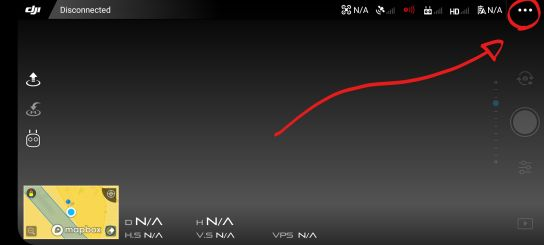
\includegraphics{images/DJI-SettingsPage.jpg}
\caption{Arrow indicating settings page location}
\end{figure}

The main control settings tab allows the user to modify a number of basic settings such as

\begin{figure}
\centering
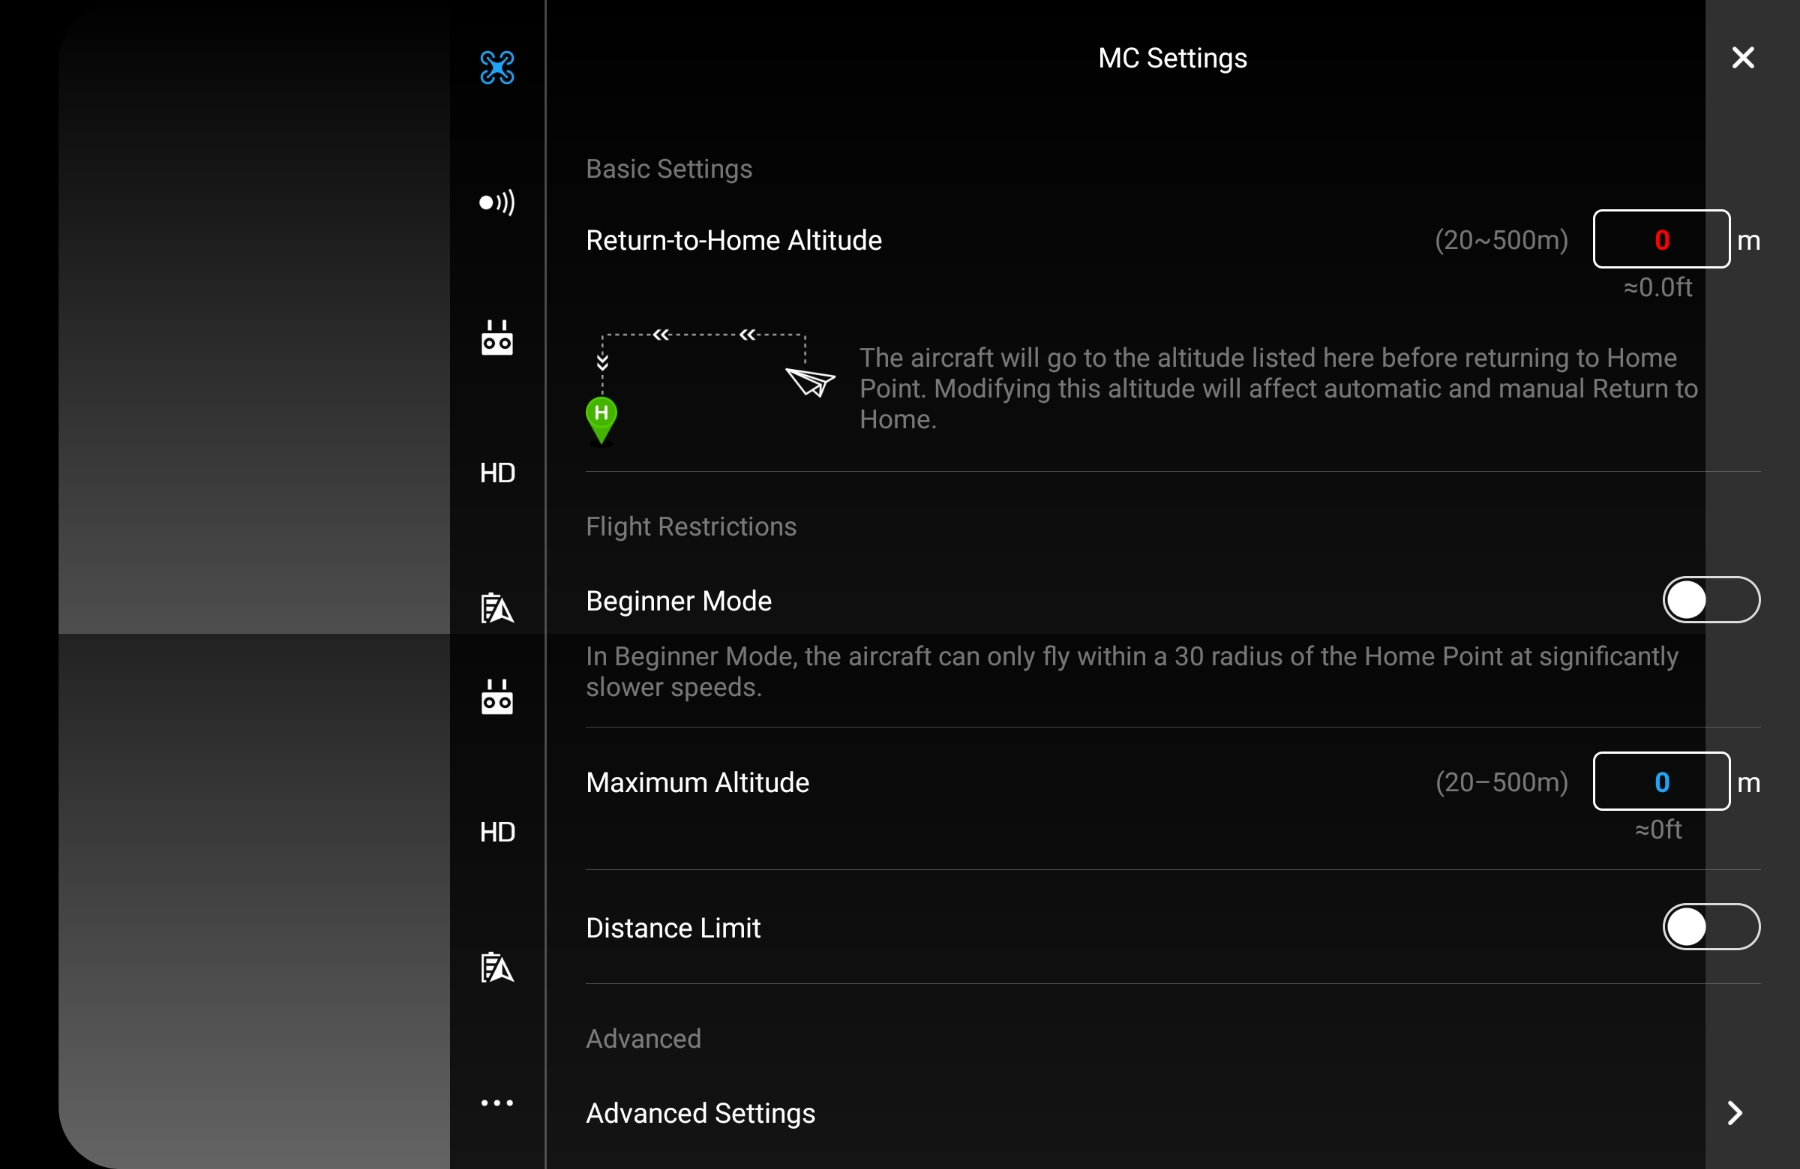
\includegraphics{images/MC/DJI-MC-SettingsPage.jpg}
\caption{Main Control Settings}
\end{figure}

\begin{enumerate}
\def\labelenumi{\arabic{enumi}.}
\tightlist
\item
  Return-to-Home Altitude
\item
  Beginner Mode
\item
  Maximum Altitude
\item
  Distance Limit
\end{enumerate}

with more advanced settings found at the bottom of the page.

\hypertarget{advanced-settings}{%
\subsection{Advanced Settings}\label{advanced-settings}}

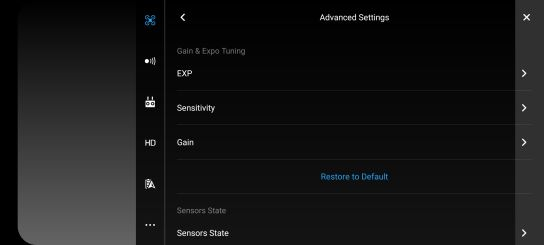
\includegraphics{images/MC/DJI-MC-Advanced-Settings.jpg}
The Advanced Settings page allows us access to a few different aircraft sensitivity settings.

\begin{enumerate}
\def\labelenumi{\arabic{enumi}.}
\tightlist
\item
  EXP
\end{enumerate}

\begin{figure}
\centering
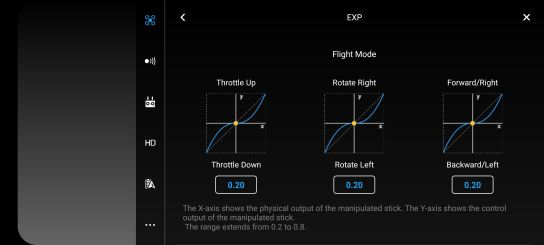
\includegraphics{images/MC/DJI-ExpSettings.jpg}
\caption{EXP settings}
\end{figure}

Tuning the EXP settings allows you to increase/decrease stick input sensitivity. The X-axis indicates user stick input and the Y-axis represents the ``value'' being output to the motors from these stick inputs. The higher the value, the more sensitive the drone can be towards the input stick movement. This is not to be confused with the next setting below.

\begin{enumerate}
\def\labelenumi{\arabic{enumi}.}
\setcounter{enumi}{1}
\tightlist
\item
  Sensitivity
\end{enumerate}

\begin{figure}
\centering
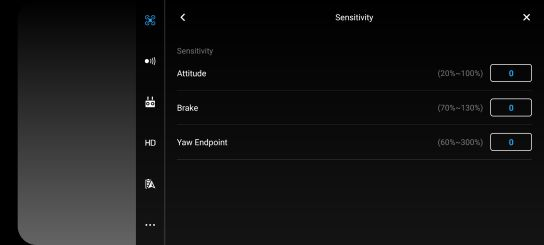
\includegraphics{images/MC/DJI-SensitivitySettings.jpg}
\caption{Sensitivity settings}
\end{figure}

The sensitivity setting affects how rapidly the drone will respond to the input. A higher value would cause the drone to react more aggressively while a lower value would dull out that same input.

\begin{enumerate}
\def\labelenumi{\arabic{enumi}.}
\setcounter{enumi}{2}
\tightlist
\item
  Gain
\end{enumerate}

\begin{figure}
\centering
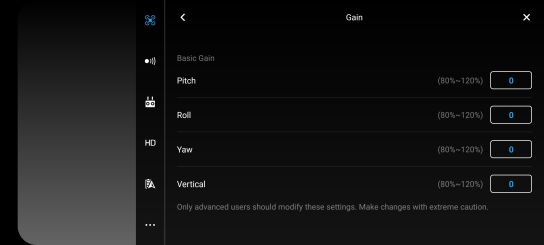
\includegraphics{images/MC/DJI-GainSettings.jpg}
\caption{Gain settings}
\end{figure}

Generally, the gain settingss are left alone.

\emph{General comment for myself, try and get a drone to checkout some of these functions before you can specifically state what it is that they do. There are some contradicting pieces of information found on the ``Gain'' settings and I don't want to give the wrong words of advice for something that can be sensitive to errors.}

\hypertarget{visual-navigation-settings}{%
\section{Visual Navigation Settings}\label{visual-navigation-settings}}

\begin{figure}
\centering
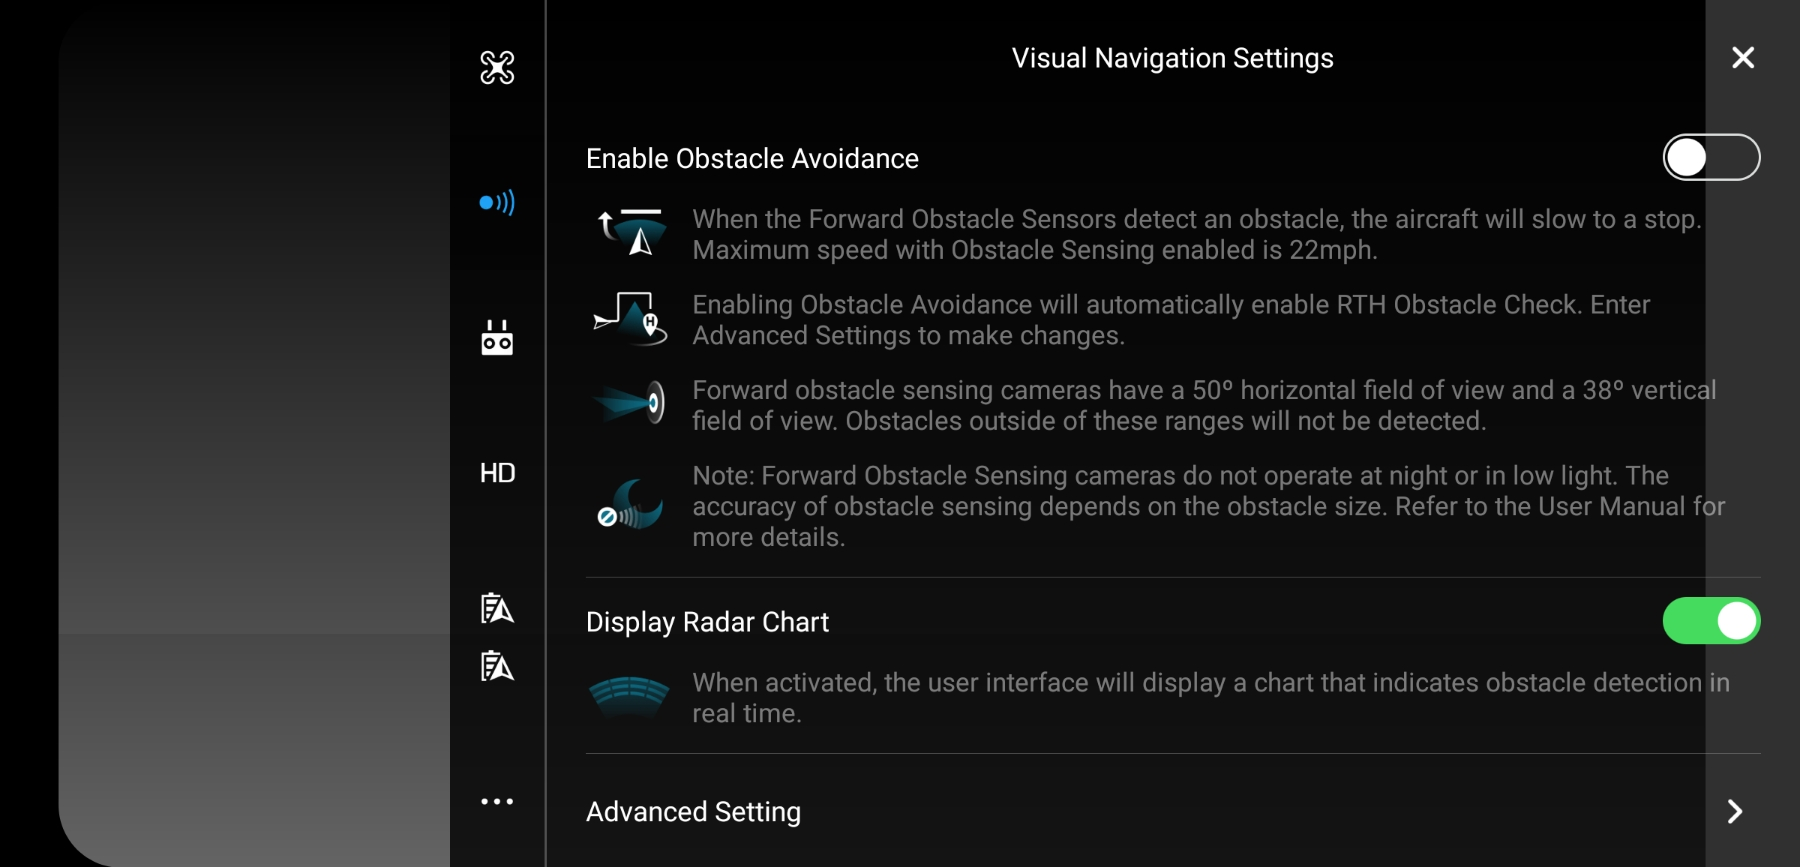
\includegraphics{images/VN/DJI-VisualNavigationSettings.jpg}
\caption{Visual Navigation Settings Page}
\end{figure}

Here we can toggle the Obstacle avoidance on and off, as well as the Radar Chart that displays real time obstacle detection. At the bottom we can again find Advanced Settings that pertain to the systems Visual navigation.

\begin{figure}
\centering
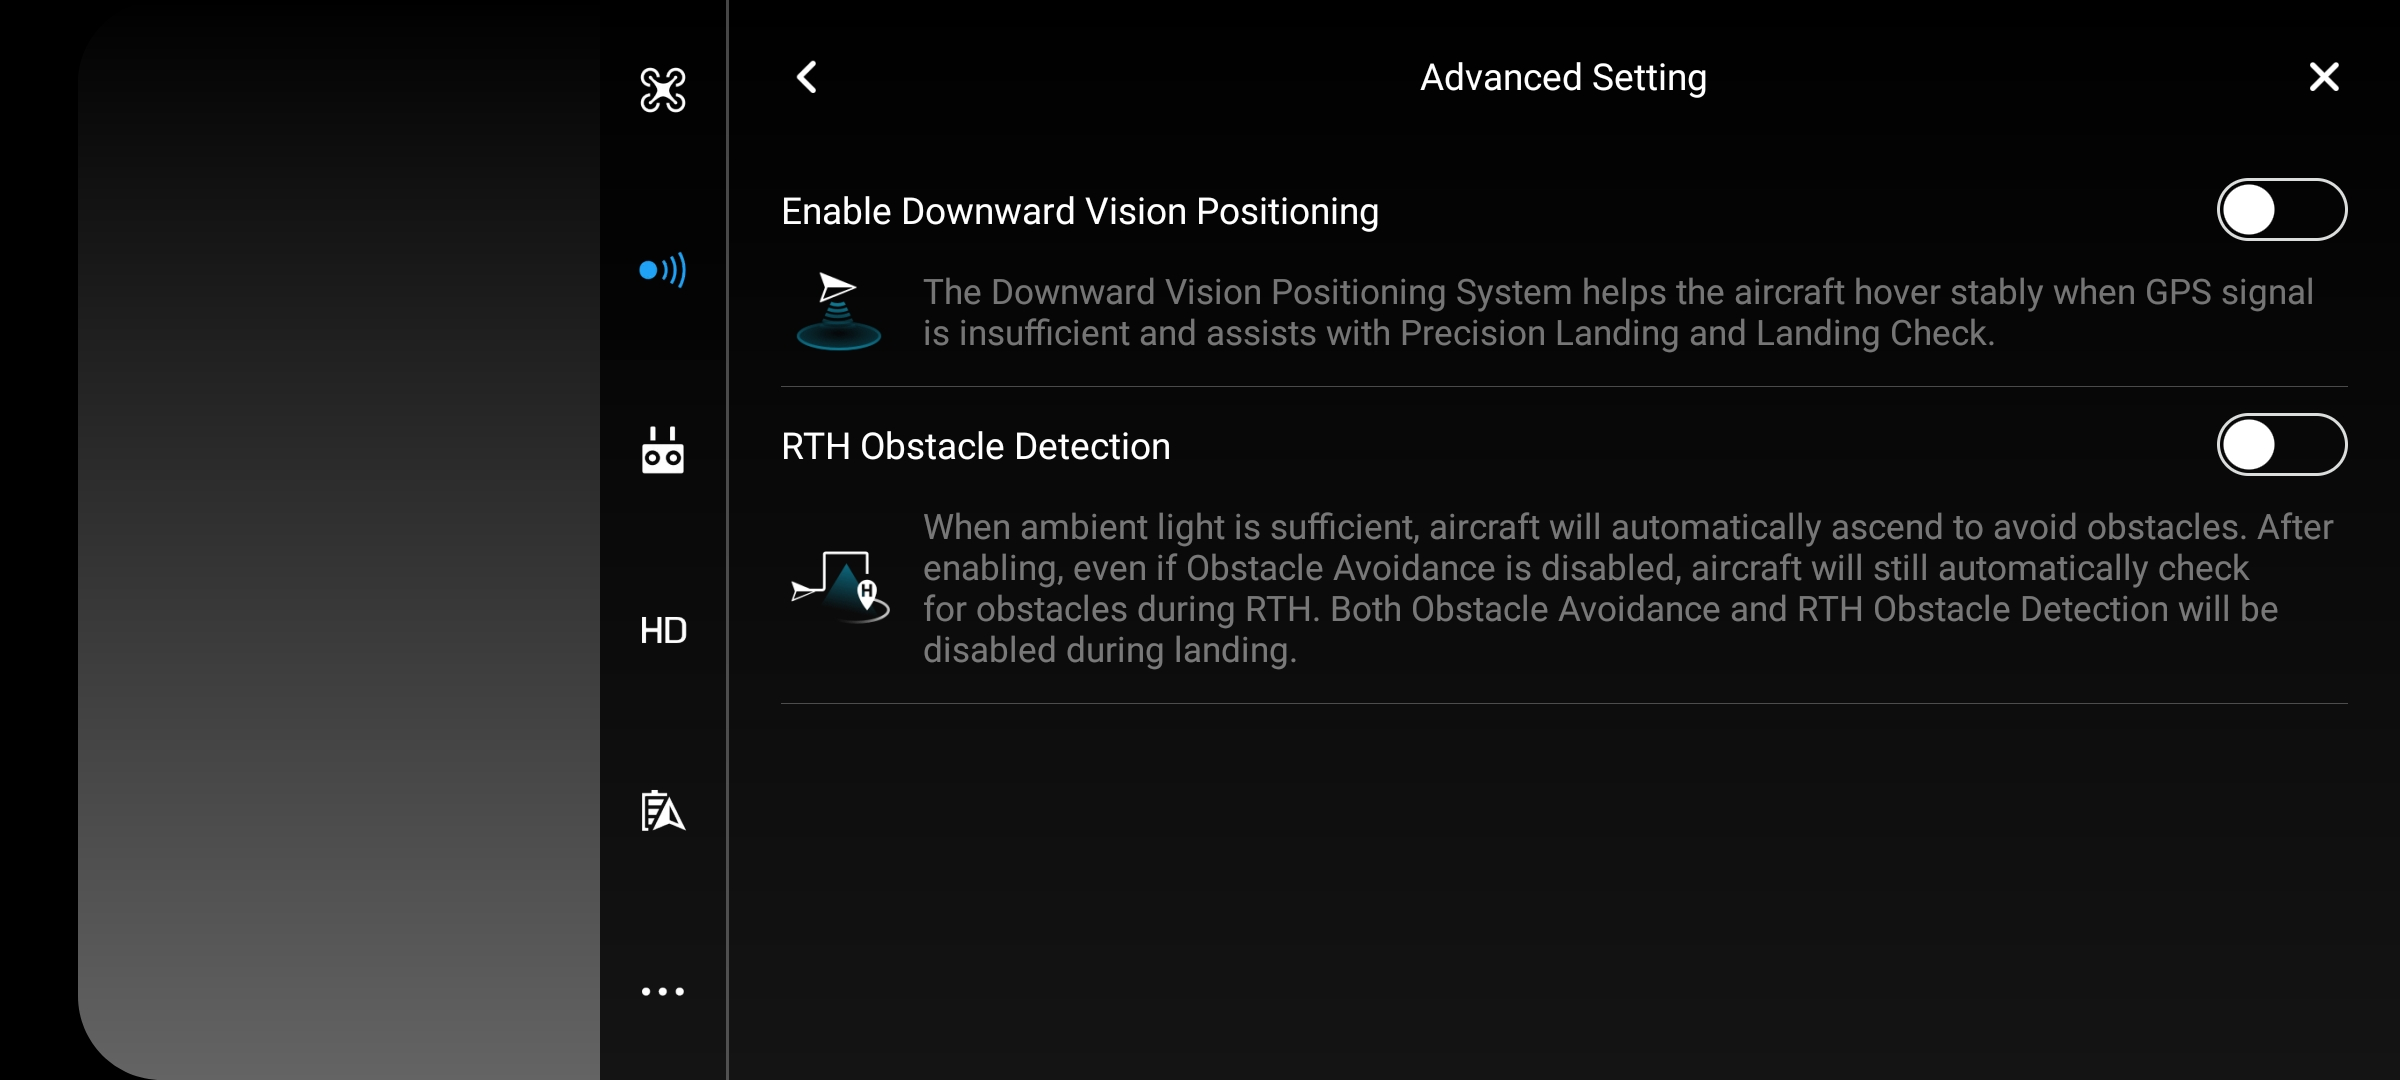
\includegraphics{images/VN/DJI-VN-AdvancedSettings.jpg}
\caption{Advanced Settings}
\end{figure}

The Advanced Settings for the Visual Navigation Settings allow for the enabling/disabling of both the Downward vision positioning system and the return-to-home obstacle detection feature.

\end{document}
